\begin{frame}\frametitle{Quark-Photon Vertex}
\begin{minipage}[r]{0.49\textwidth}
	\hspace{2mm}
	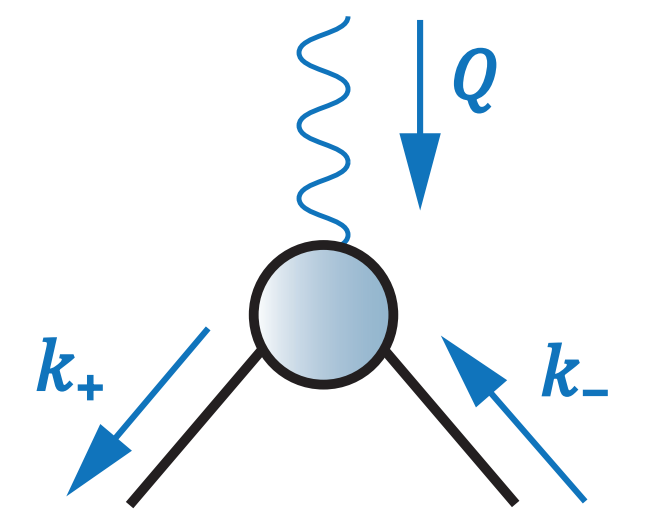
\includegraphics[height=2.2cm, width=3.2cm]{Vertex.png}
\end{minipage}
%
\begin{minipage}[r]{0.49\textwidth}
\begin{align}
k_{\pm} =& k \pm \frac{Q}{2} \\\nonumber
k_{\pm}^2=& k² \pm \frac{Q^2}{4} \pm Q\cdot k
\end{align}
\end{minipage}\\
%
\vspace{3mm}
%

In general, quarks are not on-shell \\
\hspace{2cm}$\Rightarrow$ $3$ Lorentz invariants ($Q^2, k^2, Q\cdot k$)\\
\vspace{2mm}
\hspace{2cm}$\Rightarrow$ $12$ Lorentz-Dirac tensors.\\
\vspace{2mm}
\hspace{2cm}$\Rightarrow$ $12$ dressing functions $F_i(k^2, k\cdot Q, Q^2)$
\end{frame}

\begin{frame}\frametitle{Quark-Photon Vertex}
The quark-photon vertex must satisfy electromagnetic gauge invariance in the form of the
Ward-Takahashi identity (WTI):

\begin{equation}
	Q^\mu\Gamma^\mu(k, Q)=S(k_+)^{-1}-S(k_-)^{-1}
\end{equation}

\begin{minipage}[r]{0.65\textwidth}
	$\rightarrow$ Split vertex in transverse and longitudinal parts $T_i^{\mu} \; \text{and} \; G_j^{\mu} $ with respect to incoming photon momentum:
\end{minipage}
\begin{minipage}[r]{0.30\textwidth}
	\hspace{2mm}
	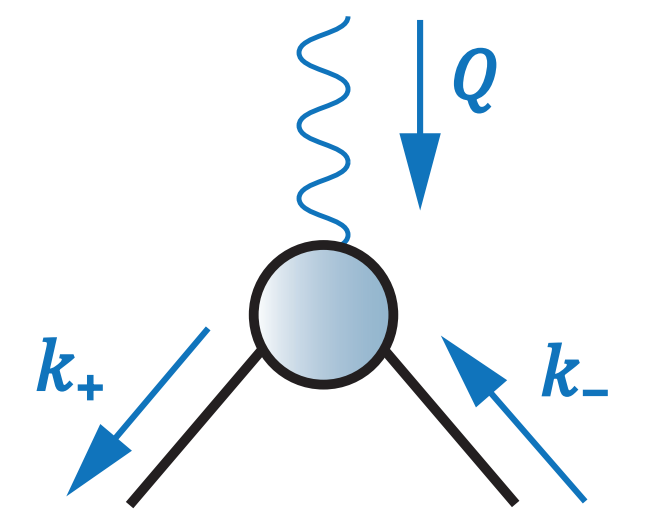
\includegraphics[height=2.2cm, width=3.2cm]{Vertex.png}
\end{minipage}

\begin{equation}
	\Gamma^\mu(k,Q)=\sum_{j=1}^4 g_j(k^2, \omega, Q^2)iG^\mu_j(k, Q)+\sum_{j=1}^8 f_j(k^2, \omega, Q^2)iT^\mu_j(k, Q)
\end{equation}

\end{frame}



\begin{frame}\frametitle{Quark-Photon Vertex}

With this decomposition, the WTI takes the easy form 
%
\begin{align}
g_1 &= \Sigma_A && g_2=2\Delta_A \\\nonumber
g_3&= 2\Delta_B && g_4=0
\end{align}
%
with 
%
\begin{align}
\Sigma_A&=\frac{A(k_+^2) + A(k_-^2)}{2} \\\nonumber
\Delta_f&=\frac{f(k_+^{2}) - f(k_-^2)}{k_+^2 - k_{-}^2} && f\, \epsilon \, \lbrace A,B \rbrace 
\end{align}
%
$\rightarrow g_j$'s are completely determined by the Quark propagator!

\end{frame}


\endinput
